%%
%% ju_liu_presentation.tex
%% 
%% Made by ju
%% Login   <ju@ubuntu>
%% 
%% Started on  Tue Aug 25 13:37:40 2009 ju
%% Last update Tue Aug 25 13:37:40 2009 ju
%%

\documentclass{beamer}

\usepackage{beamerthemesplit}
\usepackage[english]{babel}
\usepackage[latin1]{inputenc}
\setbeamercovered{transparent}

\title{GMPLS multi-layer path computation}
\author{Ju Liu -- Acreo AB}
\date{\today}

\begin{document}

\frame{\titlepage}

\section[Outline]{}
\frame{\tableofcontents}

\section{Introduction}
\subsection{Overview of the problem}
\frame
{
  \frametitle{What is the problem?}

  \begin{itemize}
  \item<1-> One billion Internet users.
  \item<2-> A lot of services are requested, like P2P, IPTV and VoIP.
  \item<3-> The network resources of the Internet Service Providers
    are under heavy stress.
  \end{itemize}
}
\frame
{
  \frametitle{What are the demands?}

  The ISPs need to:  
  \begin{itemize}
  \item<1-> Control the traffic flows and react dynamically to the
    changes in the network topology.
  \item<2-> Enable reliable automatic service provisioning throughout
    the entire network.
  \item<3-> Ensure a suitable Quality of Service for each type of
    service.
  \item<4-> \textbf{Traffic Engineering}.
  \end{itemize}
}
\subsection{Traffic Engineering}
\frame
{
  \frametitle{Traffic Engineering}

  Explicit routes:
  \begin{itemize}
  \item Traffic sharing and load balancing.
  \item Backup paths and error recovery mechanisms.
  \end{itemize}

  \begin{figure}[!hbp]
    \centering
    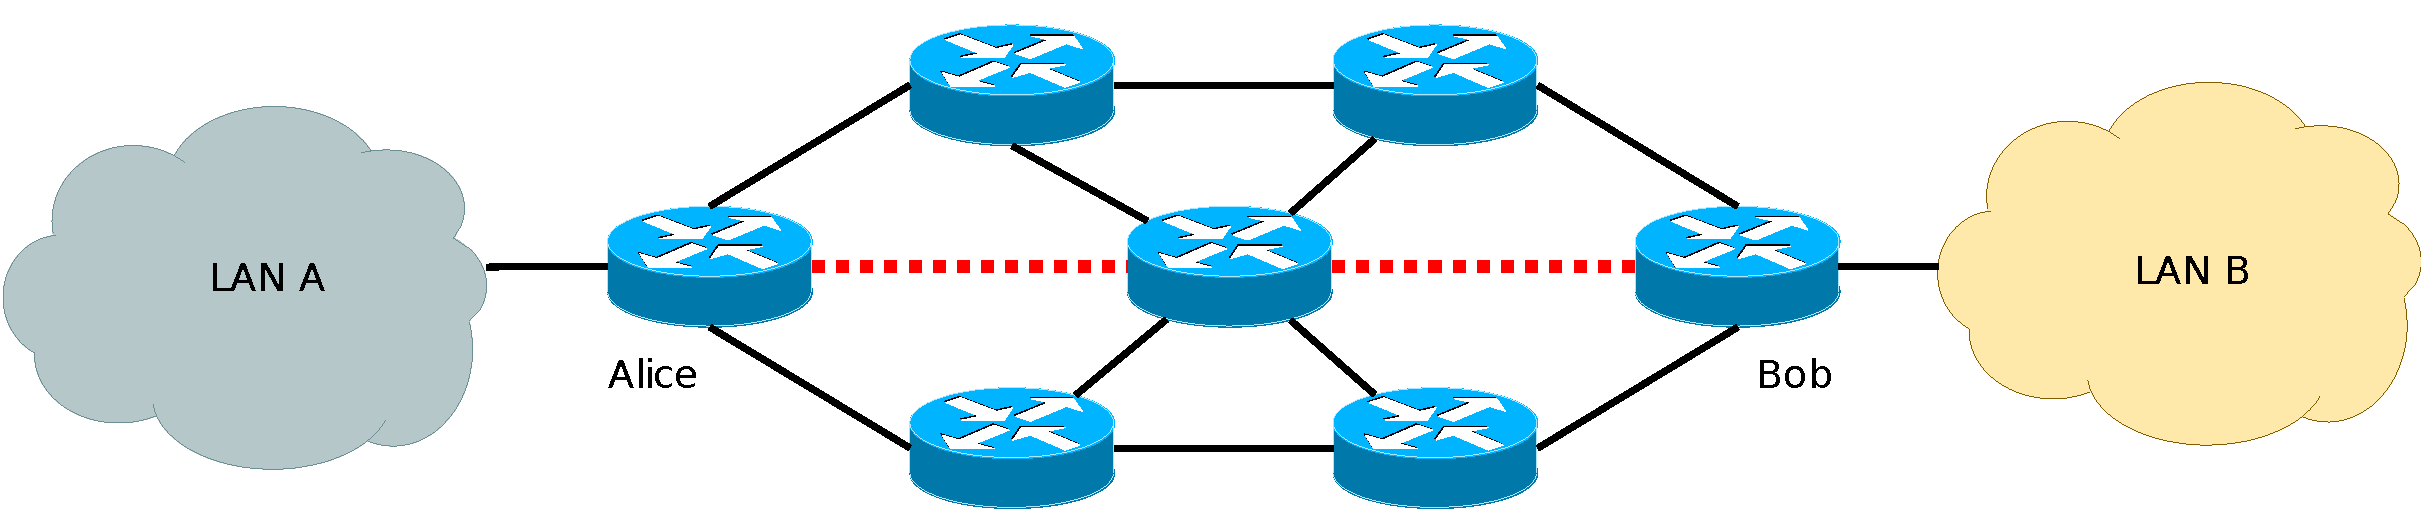
\includegraphics[width=1\textwidth]{img/mpls_te}
  \end{figure}
}
\frame
{
  \frametitle{Traffic Engineering}

  Constraint based routing:
  \begin{itemize}
  \item The shortest path is not always the best.
  \item Multiple constraints have to be considered at the same time.
  \item Different services may need different constraints.
  \end{itemize}

  \begin{figure}[!hbp]
    \centering
    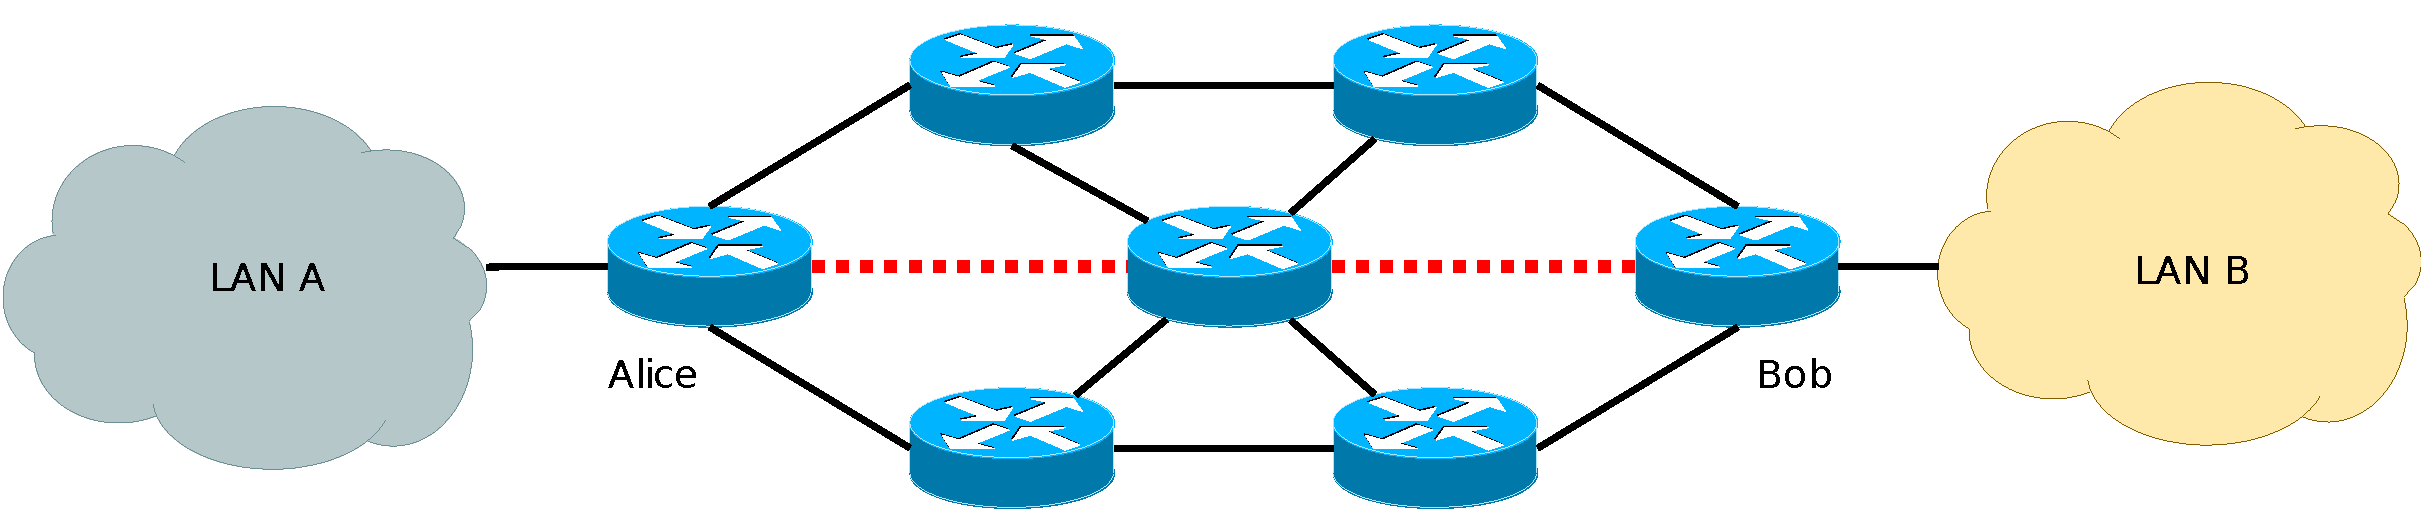
\includegraphics[width=1\textwidth]{img/mpls_te}
  \end{figure}
}

\section{What is GMPLS}
\subsection{GMPLS concepts}
\frame
{
  \frametitle{Label switching}

  \begin{itemize}
  \item<1-> A labeled packet enters in router from one interface.
  \item<2-> Depending from the label and from the incoming interface, a new
    label and an outgoing interface are chosen.
  \item<3-> The label is swapped and the packet forwarded.
  \end{itemize}
  
  \begin{figure}[!hbp]
    \centering
    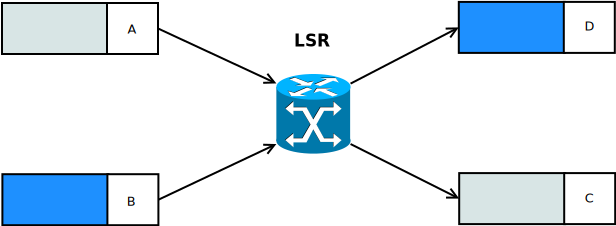
\includegraphics[width=0.7\textwidth]{img/label_switching}
  \end{figure}
}
\frame
{
  \frametitle{GMPLS definition}

  Generalized Multi-Protocol Label Switching (\textbf{GMPLS}) is suite
  of protocols designed to extend the concept of label switching to
  various transport network technologies.

}
\frame
{
  \frametitle{GMPLS protocols}
  
  The most important protocols extended in GMPLS are:
  \begin{itemize}
  \item \textbf{routing protocols}, which manage information about the
    network topology, i.e.\ IS-IS and OSPF-TE.
  \item \textbf{signaling protocols}, which manage the reservation of
    network resources and guarantee a certain QoS, i.e.\ CR-LDP and
    RSVP-TE.
  \item \textbf{link management protocols}, like LMP, which task is to
    discover and verify the connectivity of the links. 
  \end{itemize}
}
\frame
{
  \frametitle{Control and data plane}

  \begin{itemize}
  \item<1->The great innovation brought in by GMPLS is the complete
    separation of the control plane and the data plane: the former is
    used to control the setup of end-to-end connections, while the
    latter is used to actually transfer the data.
  \item<2-> While the control plane is common to every different
    technology and remains IP-based, the data plane can now diversify
    and support multiple types of switching: packets, frames,
    time-slots, wavelengths and fibers can be present at the same time
    in a GMPLS network.
\end{itemize}
}
\frame
{
  \frametitle{Switching capabilities}

  Therefore, a GMPLS network device can be:
  \begin{itemize}
    \item \textbf{Packet Switch Capable} (PSC):\\
      Router/ATM Switch/Frame Reply Switch
    \item \textbf{Time Division Multiplexing Capable} (TDMC):\\
      SONET/SDH ADM/Digital Cross-Connect
    \item \textbf{Lambda Switch Capable} (LSC):\\
      Optical ADM/Optical Cross-Connect
    \item \textbf{Fiber Switch Capable} (FSC)
  \end{itemize}
}
\frame
{
  \frametitle{An example of a multi-layer path}

  \begin{figure}[!htbp]
    \begin{center}
      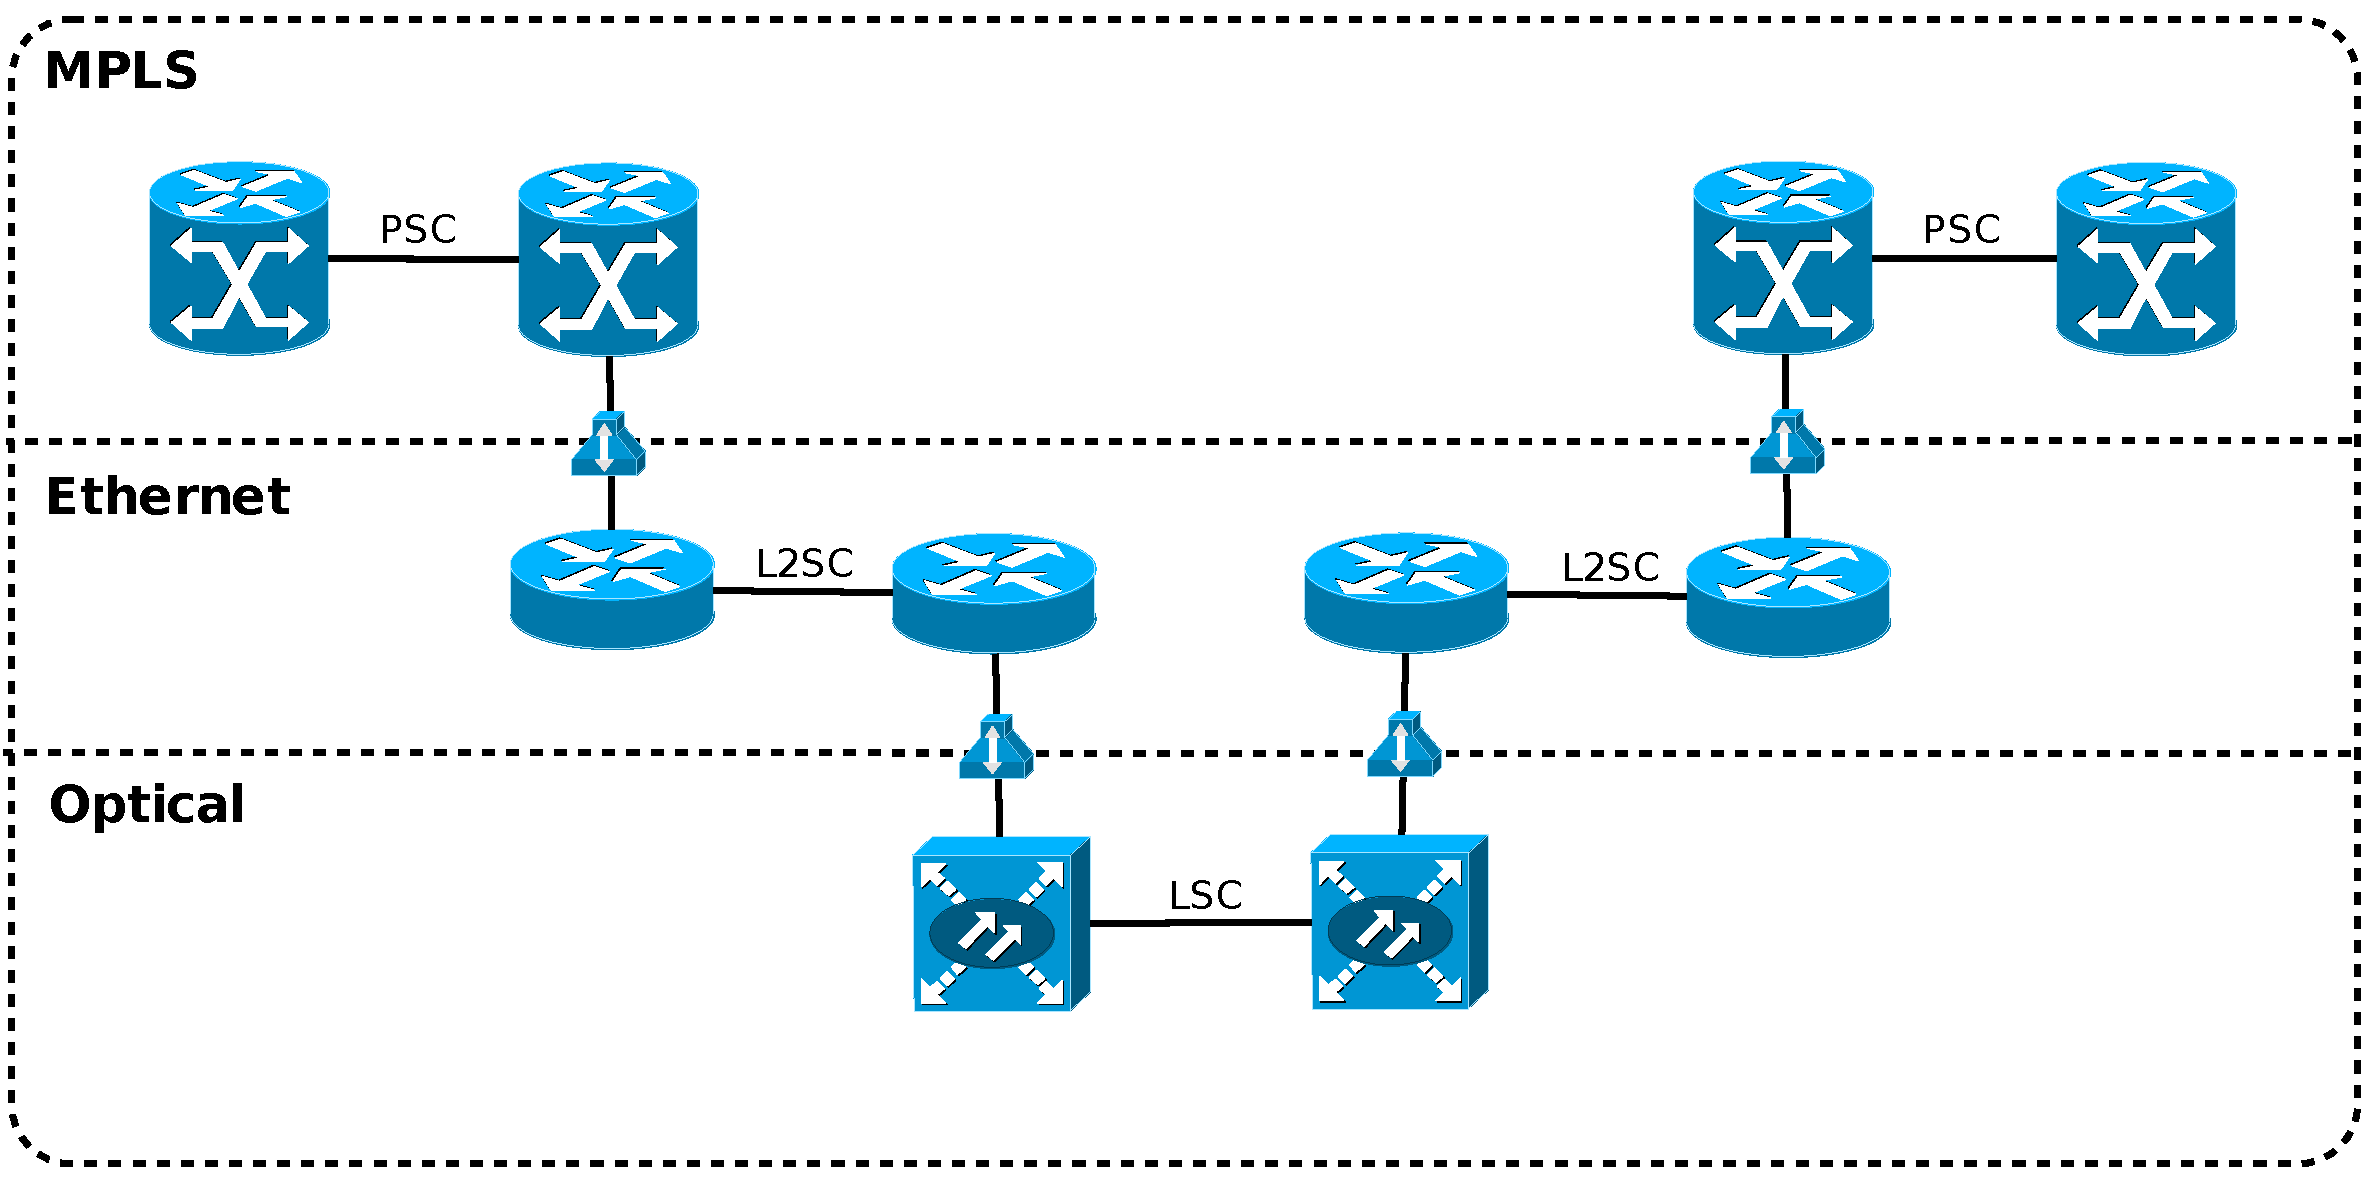
\includegraphics[width=1\textwidth]{img/multi_path}
    \end{center}
  \end{figure}
}
\frame
{
  \frametitle{GMPLS tunneling}
  
  The hierarchy of the tunnels has to be based on the natural
  difference in granularity of the different network technologies:
  packets are nested in a time-slot, time-slots are grouped in a
  wavelength and wavelengths are gathered in a fiber.

}
\frame
{
  \frametitle{The tunnels hierarchy}

  \begin{figure}[!htbp]
    \centering
    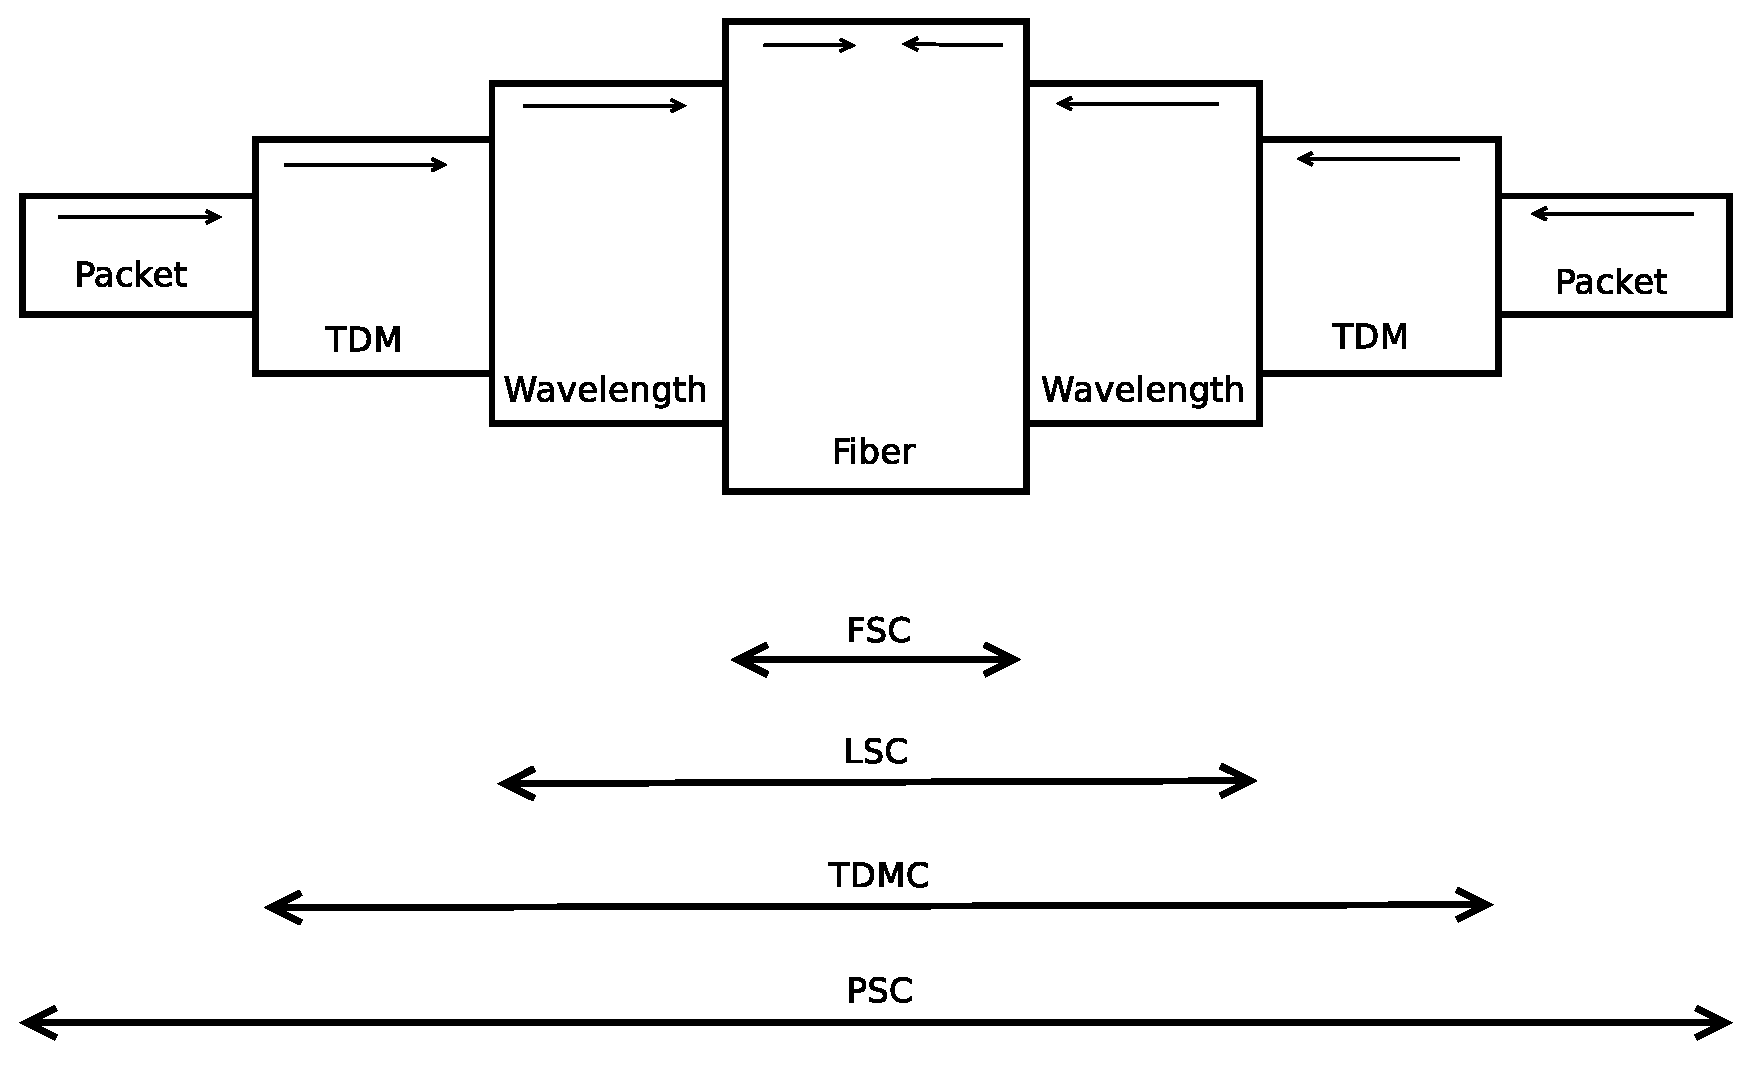
\includegraphics[width=0.9\textwidth]{img/gmpls_hierarchy}
  \end{figure}
}

\section{Software Implementation}
\subsection{The DRAGON suite}
\frame 
{ 
  \frametitle{The DRAGON suite}

  The Dynamic Resource Allocation via GMPLS Optical Networks
  (\textbf{DRAGON}) software suite is a open source GMPLS suite, which
  goal is to prove the power and the flexibility of multi-layer
  networks in order to enable dynamic end-to-end service provisioning.

}
\frame
{
  \frametitle{DRAGON architecture}

  \begin{figure}[!htbp]
    \begin{center}
      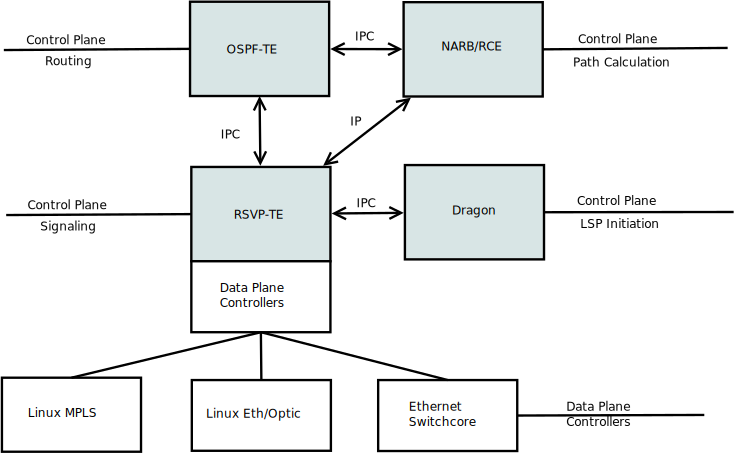
\includegraphics[width=0.9\textwidth]{img/dragon_model}
      \label{fig:dragon_model}
    \end{center}
  \end{figure}
}
\frame
{
  \frametitle{RCE architecture}

  \begin{figure}[!htbp]
    \begin{center}
      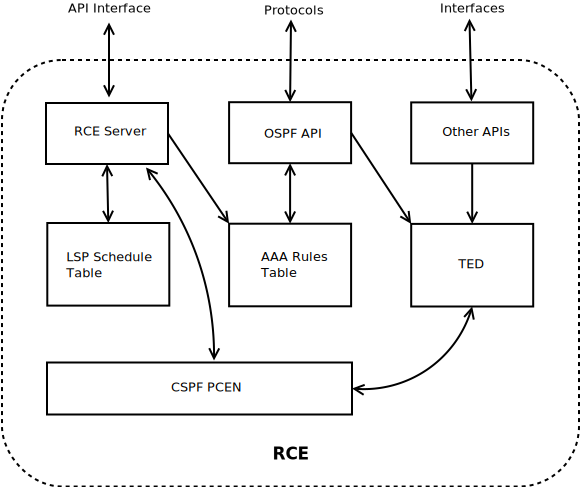
\includegraphics[width=0.65\textwidth]{img/rce_model}
    \end{center}
  \end{figure}
}
\frame
{
  \frametitle{PCEN Module}
  
  \begin{figure}[!htbp]
    \begin{center}
      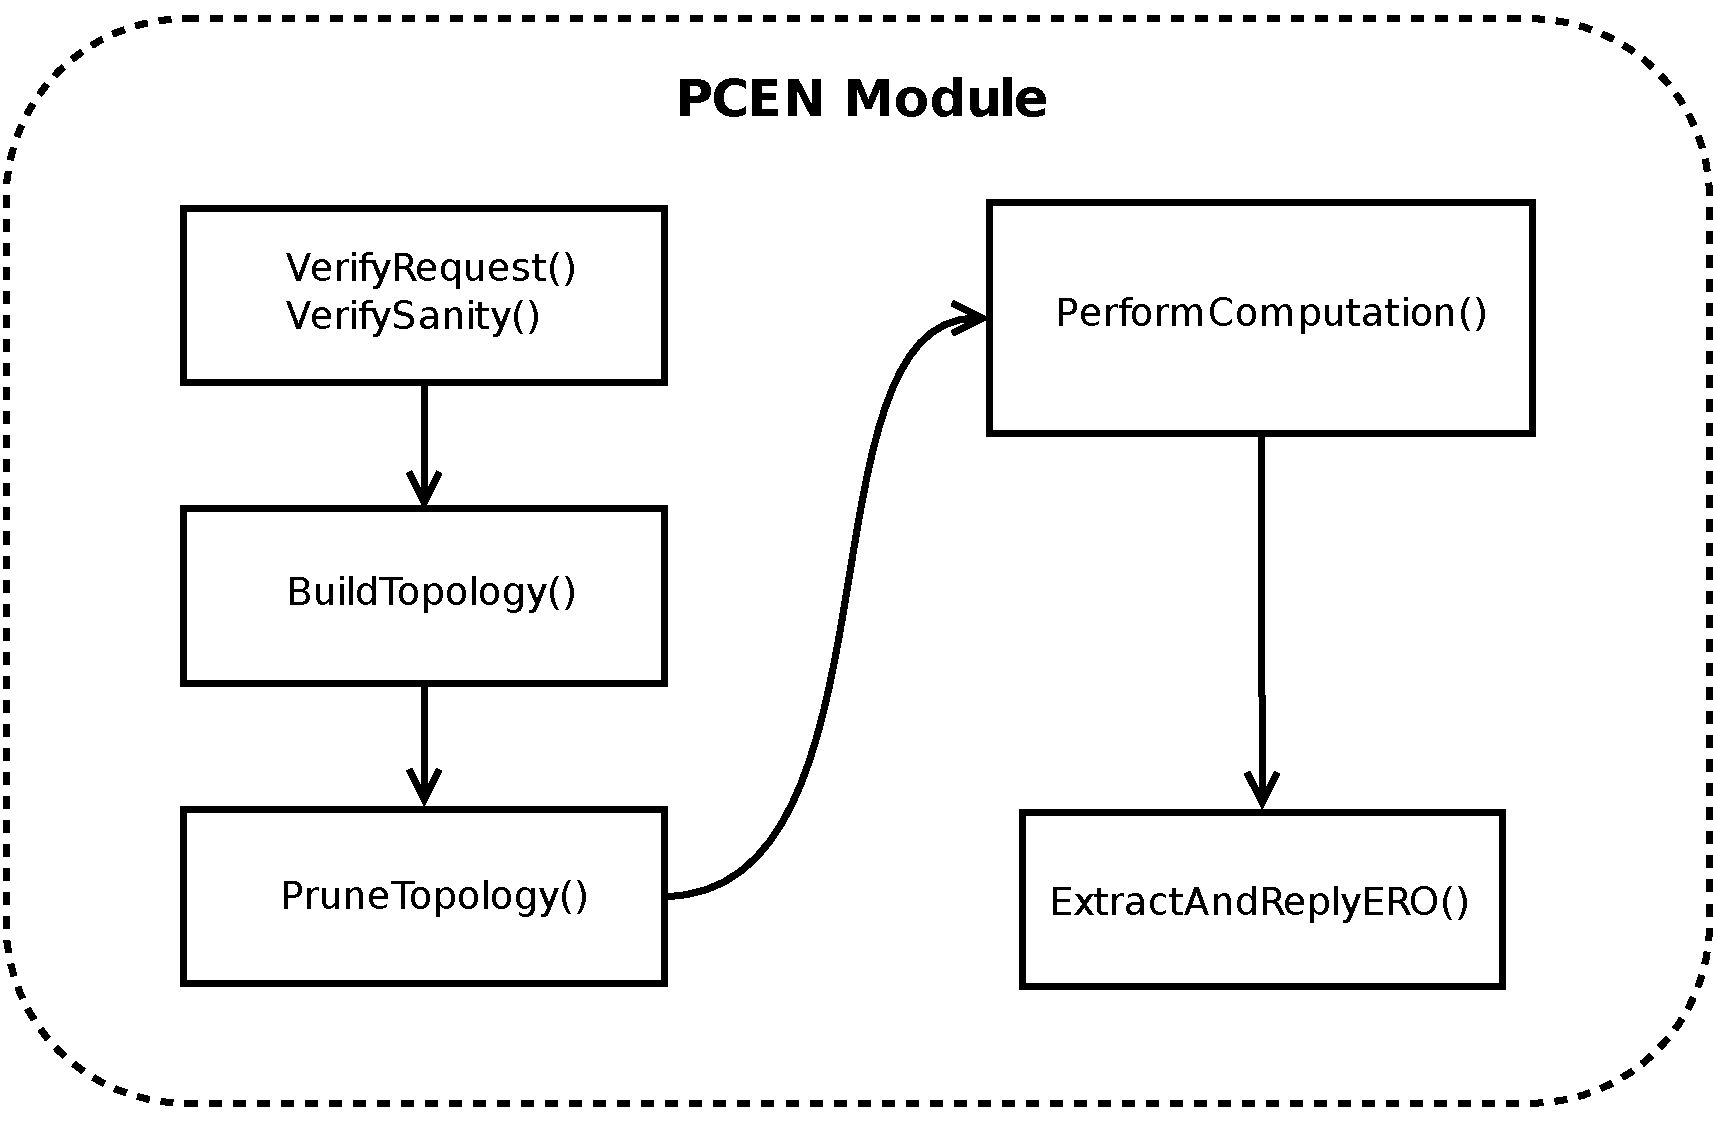
\includegraphics[width=0.8\textwidth]{img/pcen_module}
    \end{center}
  \end{figure}
}
\frame
{
  \frametitle{Candidate CSPF Algorithm}

  The implemented CSPF algorithm is derived from the BFS algorithm and
  searches for the loop-less paths between a source and a destination
  inside a multi-layer network.

  \begin{figure}[!htbp]
    \begin{center}
      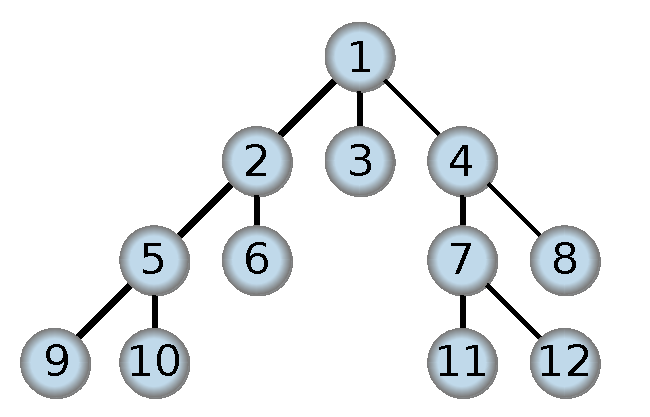
\includegraphics[width=0.5\textwidth]{img/bfs_graph}
    \end{center}
  \end{figure}
}
\frame
{
  \frametitle{Considered constraints}

  \begin{itemize}
  \item The constraints considered include general constraints, like
    bandwidth or accumulated metric, or layer-specific constraints,
    like wavelength continuity in the optical layer.
  \item A set of user-defined constraints has been supported to offer
    a better level of customization and flexibility.
  \end{itemize}
}
\frame
{
  \begin{figure}[!htbp]
    \begin{center}
      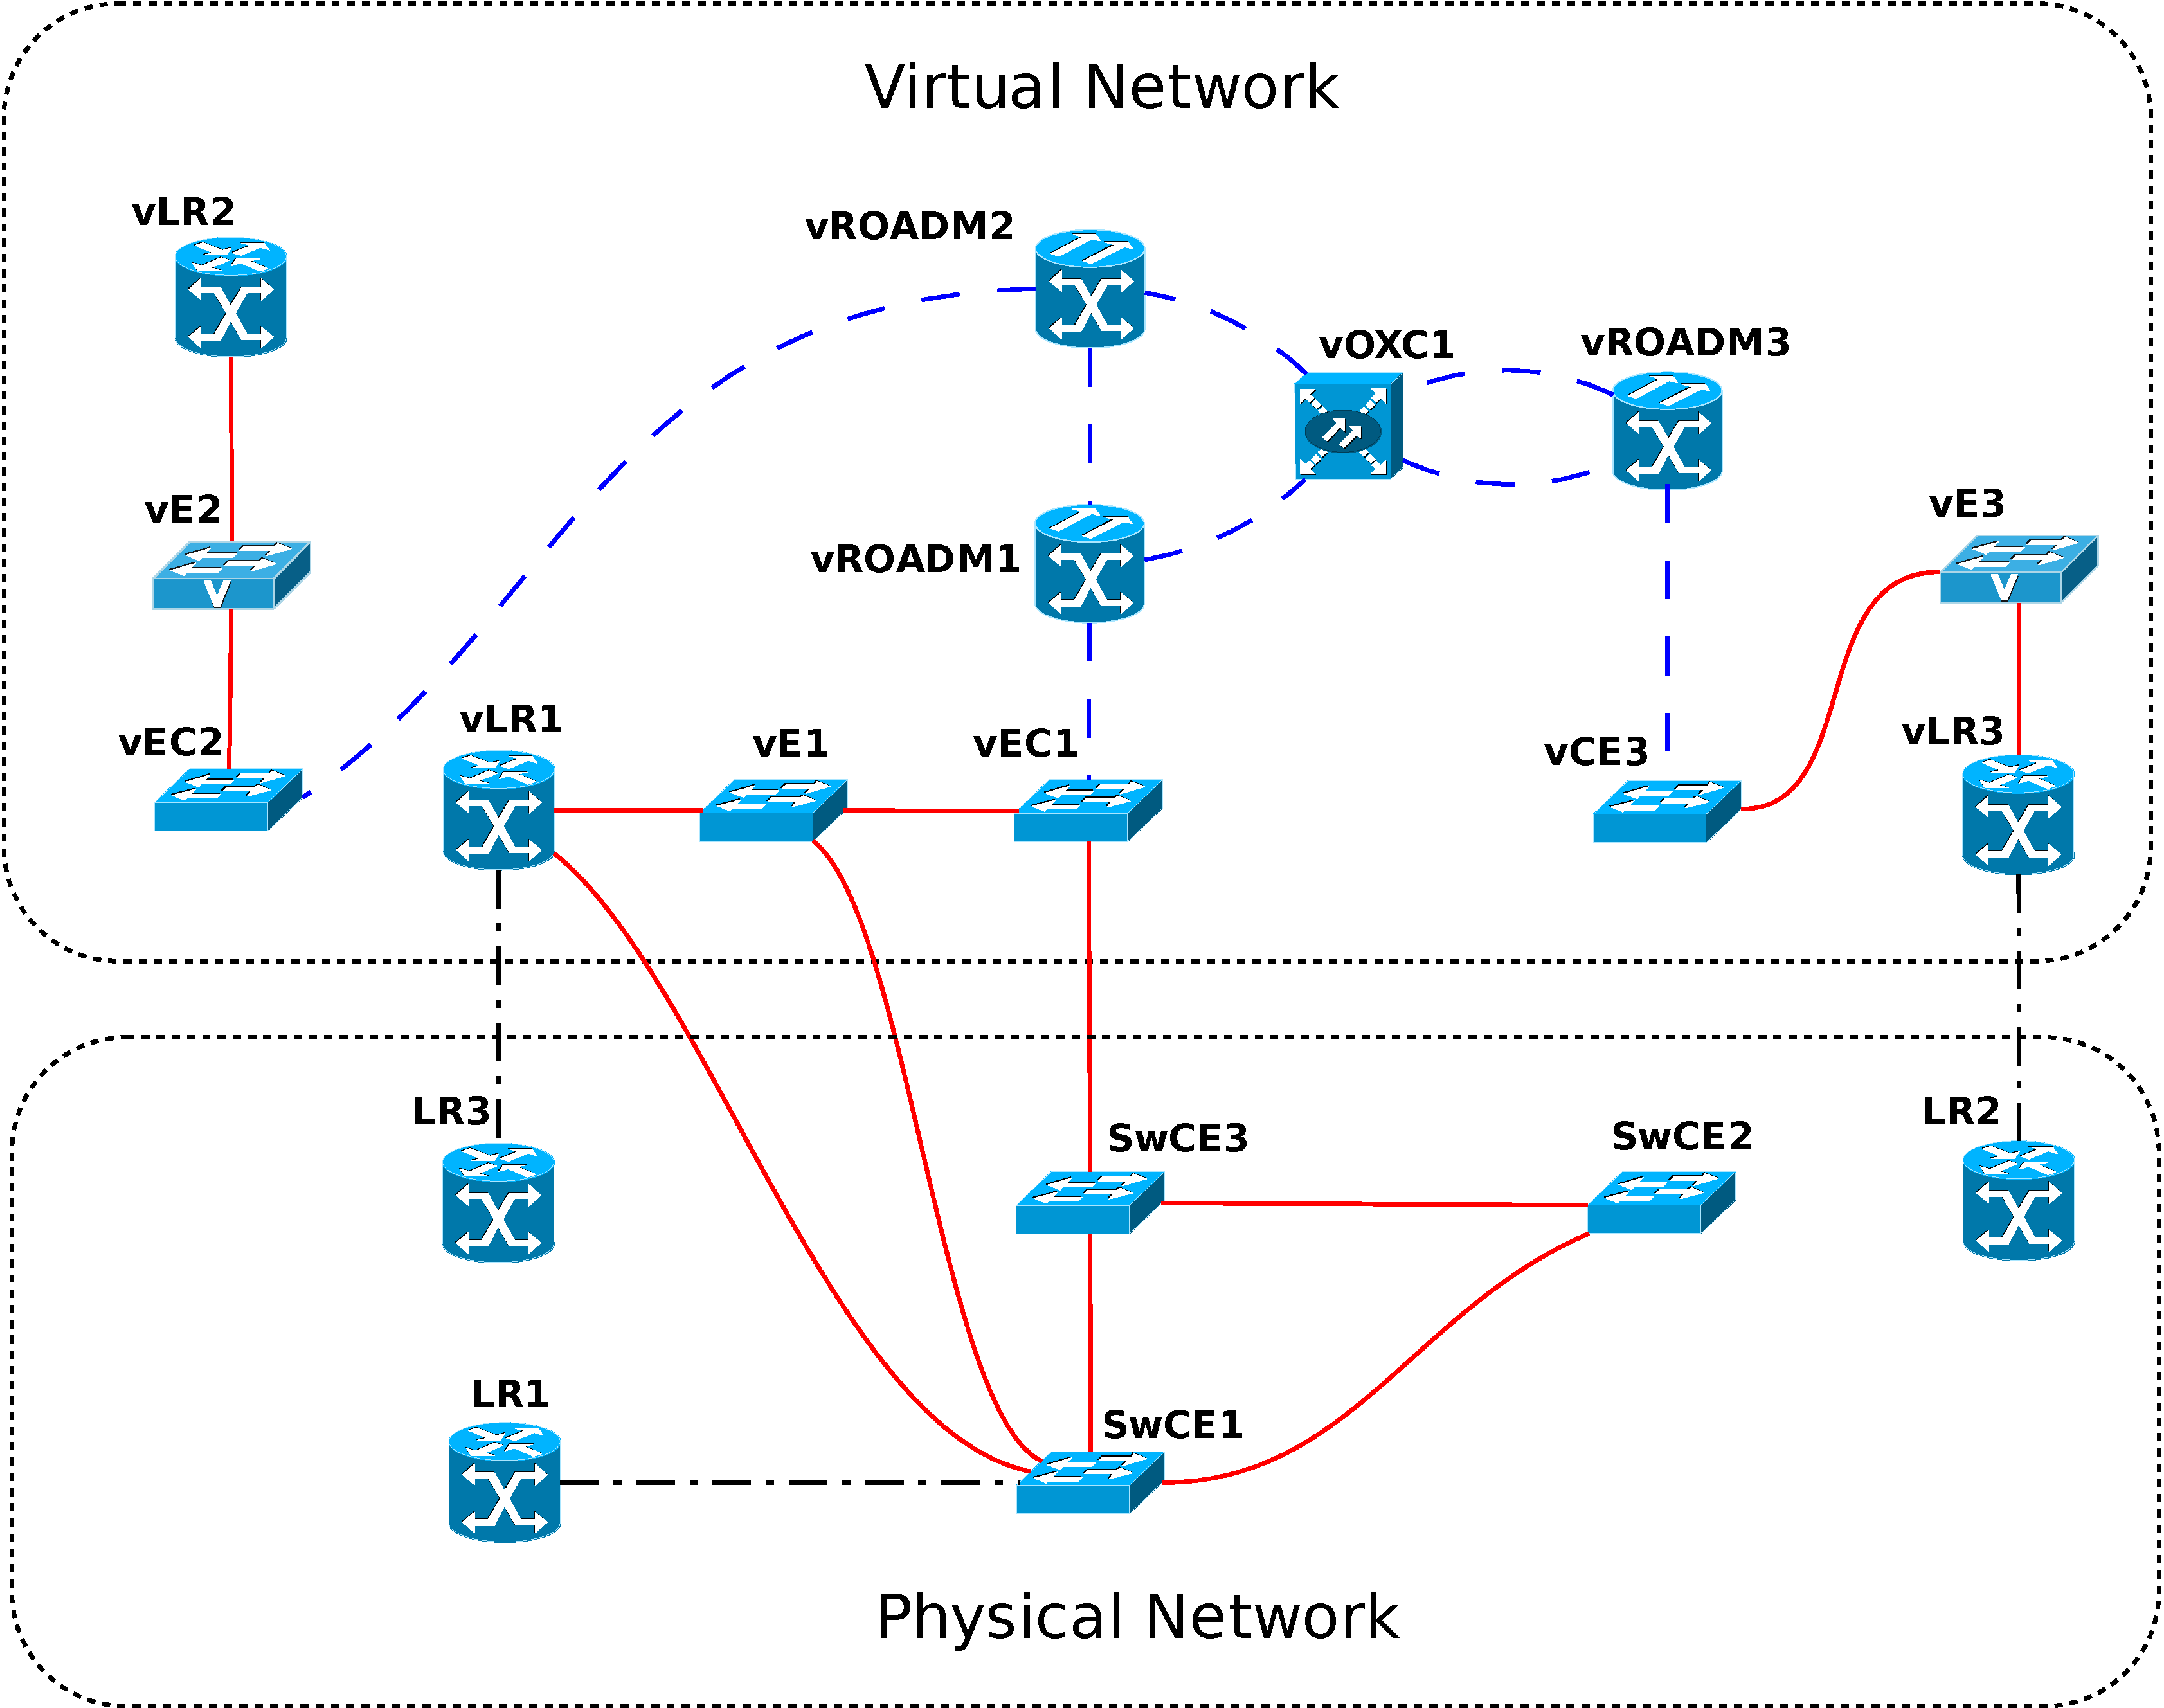
\includegraphics[width=0.8\textwidth]{img/testbed_model}
    \end{center}
  \end{figure}
}
\frame
{
  \frametitle{Example of multi-layer path}

  \begin{figure}[!htbp]
    \begin{center}
      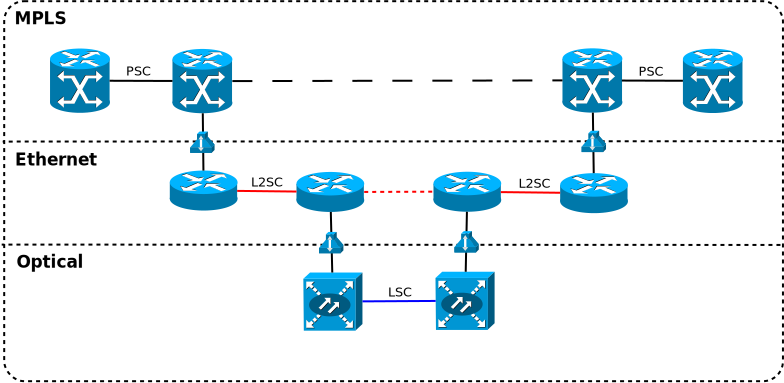
\includegraphics[width=1\textwidth]{img/multi_path2}
    \end{center}
  \end{figure}
}
\frame
{
  \frametitle{Constraints checking}

  \begin{itemize}
  \item The multiple network technologies require layer-specific
    constraints to be respected.
  \item The algorithm maintains a working set of constraints
    associated to the current layer.
  \item When starting a tunnel, the working set is ``frozen'' and a
    new set of constraints is taken into consideration.
  \item When the tunnel ends, the previous set of constraints is
    reverted and used as working set.
  \end{itemize}
}
\frame
{
  \frametitle{Test cases}

  The following tests have been setup:

  \begin{enumerate}
  \item<1-> The path computation request includes two neighbours with L2SC
    interfaces (vE1 and vEC1); the RCE doesn't need to setup LSP
    tunnels.
  \item<2-> The source and the destination requested belong to the optical
    layer and are connected through an optical cross-connect (vROADM2
    and vROADM3); the RCE needs to check for wavelength continuity but
    doesn't need to setup a tunnel.
  \item<3-> In the last case, the source and destination are at the
    opposite sides of the testbed (LR1 and LR2); the path is composed
    by a high number of hops and two nested LSP tunnels have to be
    setup by the RCE.
  \end{enumerate}
}
\frame
{
  \frametitle{Performance evaluation}

  The performance of the algorithm has been evaluated considering the
  usage of two different resources:

  \begin{itemize}
  \item \textbf{time}, intended as the response time of
    the algorithm.
  \item \textbf{space}, intended as the memory needed to run it.
  \end{itemize}

  Each of the test cases has been executed in three different runs
  with 10, 100 and 1000 iterations respectively.

}
\frame
{
  \frametitle{Time efficiency}

  The time efficiency of the algorithm has been measured starting from
  the \textbf{response time}, that is the time that passes from when
  the RCE receives the path computation request to when the RCE sends
  the computed path back to the client. The response time have been
  later divided in multiple intervals.

}
\frame
{
  \frametitle{Time efficiency summary}
  
  \begin{figure}[!htbp]
    \begin{center}
      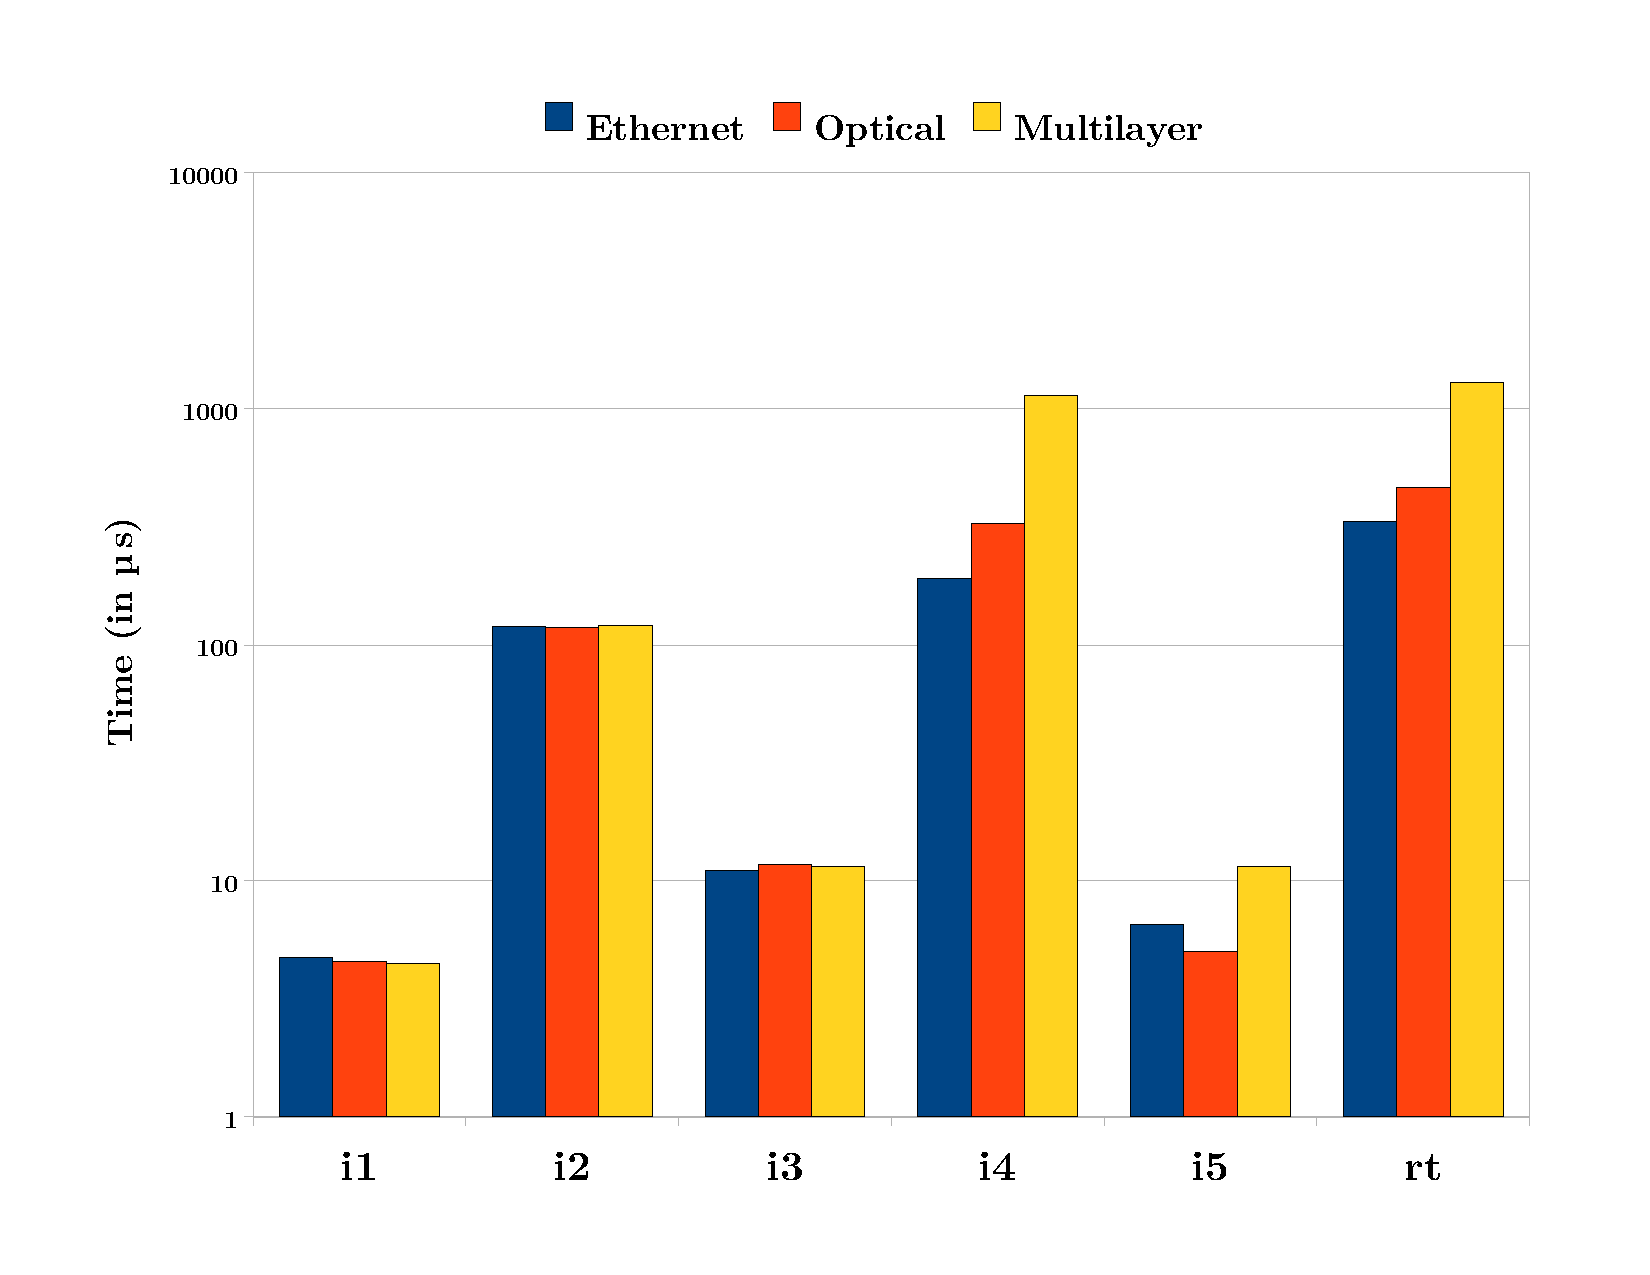
\includegraphics[width=0.75\textwidth]{img/time_graph}
    \end{center}
  \end{figure}
}
\frame
{
  \frametitle{Space Efficiency}

  The space efficiency of the algorithm has been analyzed considering
  the usage of RAM on the server; the \textit{valgrind} program has
  been used to verify the presence of memory leaks in the software
  implementation.

  \begin{itemize}
  \item The program was started to monitor the behaviour of the RCE
    and then a specific number of requests was sent from a client.
  \item When the RCE had completed to process the requests, valgrind
    was terminated to generate a memory usage report.
  \end{itemize}
}
\frame
{
  \begin{figure}[!htbp]
    \begin{center}
      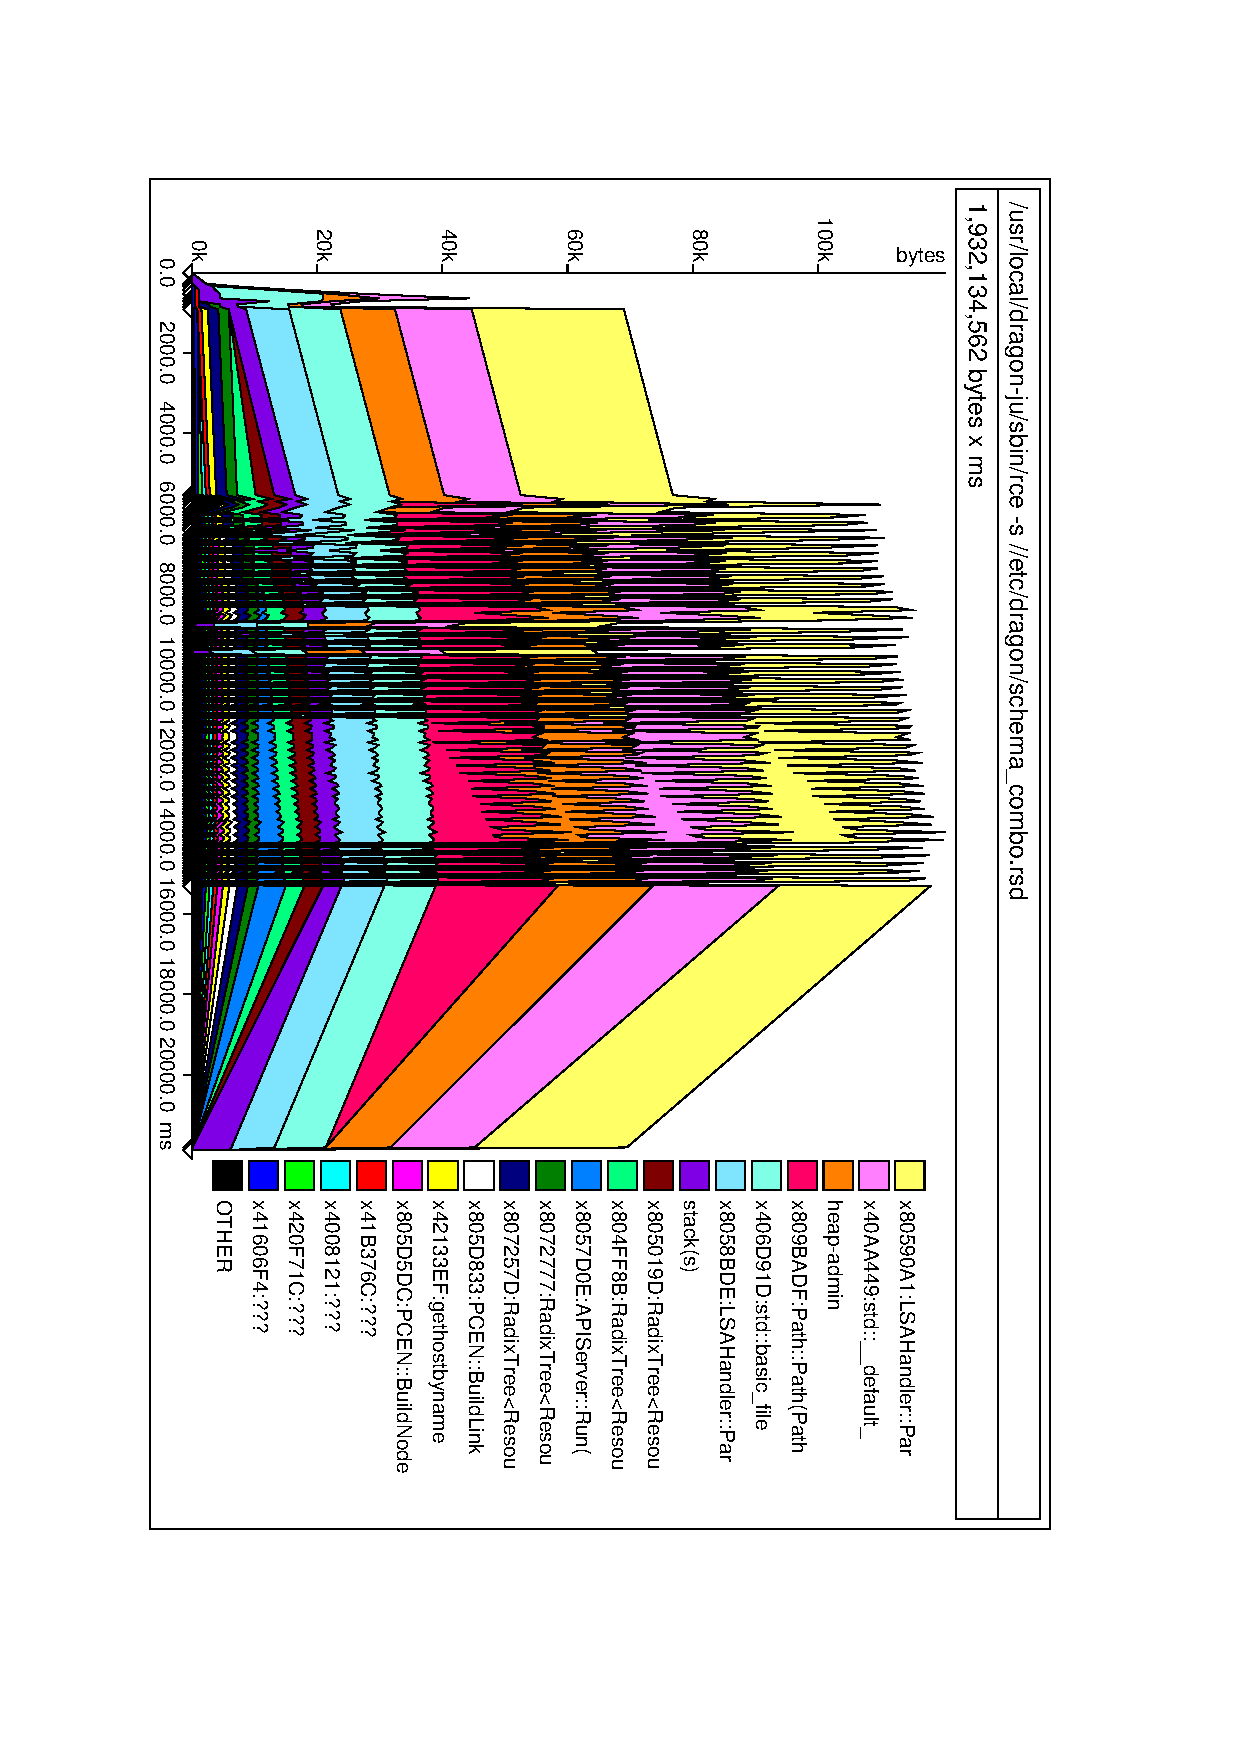
\includegraphics[width=1\textwidth]{img/multi-100}
    \end{center}
  \end{figure}
}

\section{Conclusions}
\frame
{
  \frametitle{Conclusions}

  This thesis work have been focused on the improvement of the
  automatic path-setup process in a complex multi-layered network:

  \begin{itemize}
  \item<1-> A path computation algorithm has been developed and thoroughly tested,
    proving that it is feasible to simplify the current manual process
    with a faster and more dynamic one. 
  \item<2-> The implemented solution can handle successfully a wide
    range of path constraints, showing also the capability of adapting
    itself in case of network topology changes; in addition, the support
    of user-defined constraints makes the system more flexible, allowing
    a finer degree of configuration.
  \end{itemize}
}
\frame
{
  \frametitle{The End}

  \begin{center}
  Questions?
  \end{center}
}

\end{document}

%%% Local Variables: 
%%% mode: latex
%%% TeX-master: t
%%% compile-command: "latexmk -pdf ju_liu_presentation"
%%% Local IspellDict: english
%%% End: 
